\subsection{Creating a Python list}
We can create a List in Python using 2 ways:
\begin{itemize}
	\item Using list() constructor.
	\item Using square bracket([]).
\end{itemize}
\newpage

\begin{figure}[h]
	\centering
	\begin{minipage}[t]{0.47\textwidth}
		\centering
		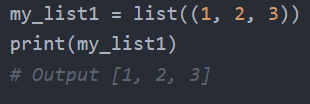
\includegraphics[width=\linewidth]{list-constructor}
		\caption{Creating list using constructor}
		\label{fig:left}
	\end{minipage}
	\hfill
	\begin{minipage}[t]{0.48\textwidth}
		\centering
		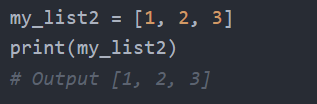
\includegraphics[width=\linewidth]{list-squarebracket}
		\caption{Creating list using square bracket}
		\label{fig:right}
	\end{minipage}
\end{figure}

\subsection{Length of a List}

{\large Definition:} Length of a List = the number of items present in a list. \\ [0.5em]
We can get the length of a List using len() function.
\begin{figure}[h]
	\centering
	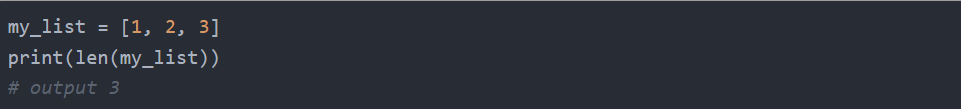
\includegraphics[width=1.0\textwidth]{list-length}
	\caption{Calculate the length of a list using len()}
	\label{fig:length}
\end{figure}

\subsection{Accessing items of a List}
{\large Items in a List could be accessed by:}
\begin{itemize}
	\item Indexing.
	\item Slicing. 
\end{itemize}
\subsubsection{Indexing}
 List is 0-indexed, which means if we want to access the 3rd element, for example, we need to use 2 since the index value starts from 0. \\ [0.5em]
 There are two types of indexing technique:
 \begin{itemize}
 	\item Positive indexing.
 	\item Negative indexing.
 \end{itemize}
 \newpage
 
\begin{figure}[h]
	\centering
	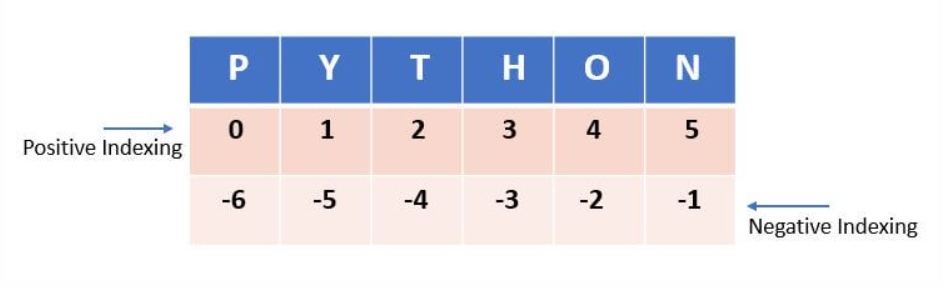
\includegraphics[width=1.0\textwidth]{indexing}
	\caption{Positive and negative indexing}
	\label{fig:indexing}
\end{figure}

{\large Common errors:} 
\begin{itemize}
	\item Access an item with an index more than Lists length, it will throw the 'Index Error'.
	\item If we give any other type except for integer for index values, then it will throw Type Error.
\end{itemize}

\begin{figure}[h]
	\centering
	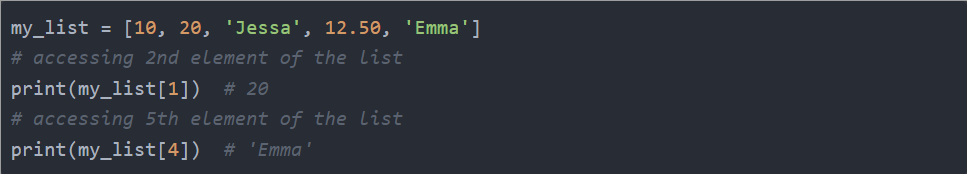
\includegraphics[width=1.0\textwidth]{pos-indexing}
	\caption{Examples of positive indexing}
	\label{fig:posindex}
\end{figure}

{\large Negative Indexing: }The elements in the list can be accessed from right to left by using negative indexing. The negative value starts from -1 to -length of the list. It indicates that the list is indexed from the reverse/backward.

\begin{figure}[h]
	\centering
	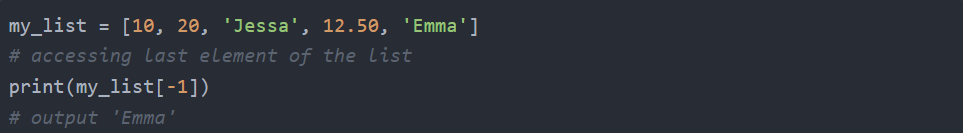
\includegraphics[width=1.0\textwidth]{negative-indexing}
	\caption{Examples of negative indexing}
	\label{fig:negindex}
\end{figure}
\newpage
\subsubsection{Slicing}
{\large Definition:} Slicing a list implies, accessing a range of elements in a list.For example, if we want to get the elements in the position from 3 to 7, we can use the slicing method. We can even modify the values in a range by using this slicing technique. \\

{\large Syntax for slicing:}

\begin{figure}[h]
	\centering
	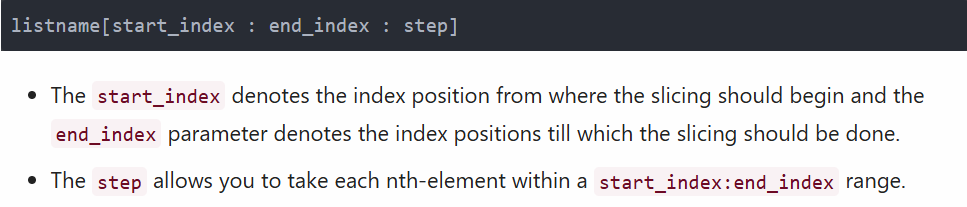
\includegraphics[width=1.0\textwidth]{slicing}
	\caption{Slicing syntax}
	\label{fig:slicing}
\end{figure}
\begin{figure}[h]
	\centering
	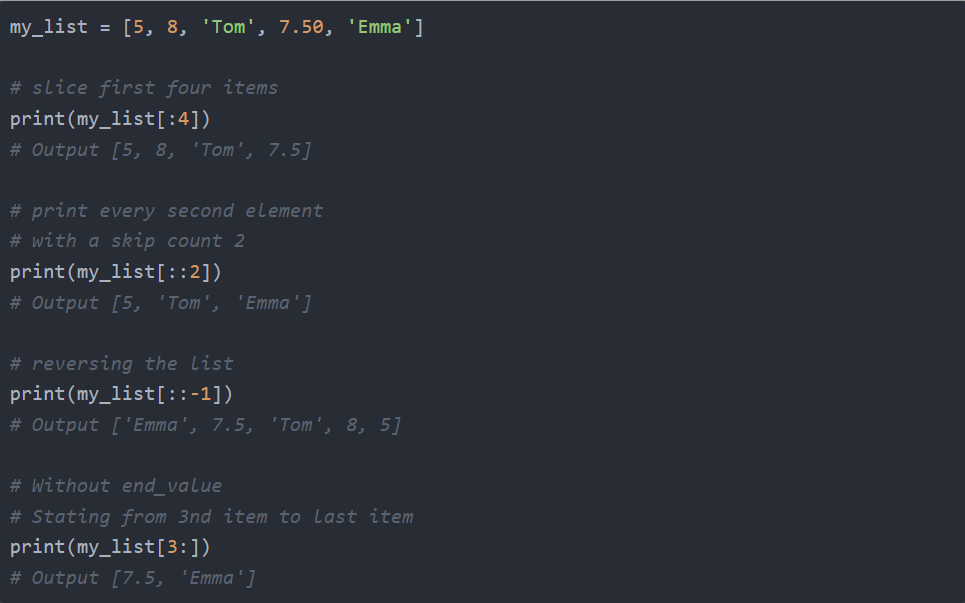
\includegraphics[width=1.0\textwidth]{slicing-example}
	\caption{Examples of slicing}
	\label{fig:sliexam}
\end{figure}

\subsection{Iterating a List}
The objects in the list can be iterated over one by one, by using a for a loop.
\newpage
\begin{figure}[h]
	\centering
	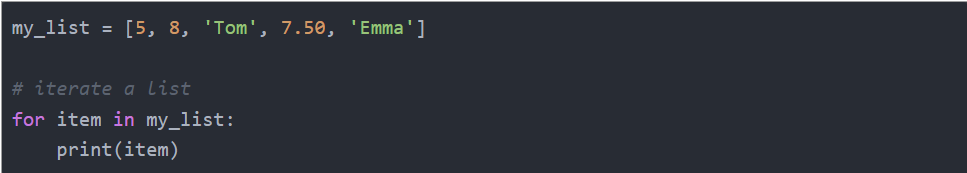
\includegraphics[width=1.0\textwidth]{list-iterate}
	\caption{List iterating example}
	\label{fig:list-iterate}
\end{figure}

\subsection{Adding elements to the List}
\begin{table}[h!]
	\centering
	\begin{tabularx}{\textwidth}{|l|l|X|}
		\hline
		\textbf{Method} & \textbf{Syntax} & \textbf{Usage} \\
		\hline
		append() & mylist.append('Emma') & Only accept one parameter and add it at the end of the list \\
		\hline
		insert() & insert(index, object) & Add the object/item at the specified position in the list \\
		\hline
		extend() & mylist.extend([25, 75, 100]) & Accept the list of elements and add them at the end of the list, We can even add another list. \\
		\hline

	\end{tabularx}
	\caption{Methods for adding elements in List}
	\label{tab:list-add-opers}
\end{table}

\subsection{Modify the items of a List}

\begin{itemize}
	\item Modify the individual item.
		\begin{figure}[h]
			\centering
			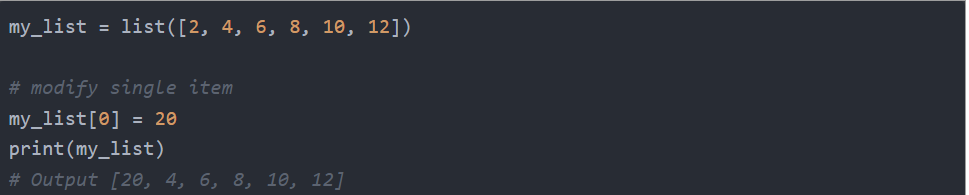
\includegraphics[width=1.0\textwidth]{single-modify-list}
			\caption{Modify a single item.}
			\label{fig:list-single-modify-list}
		\end{figure}
	\newpage
	\item Modify the range of items.
		\begin{figure}[h]
			\centering
			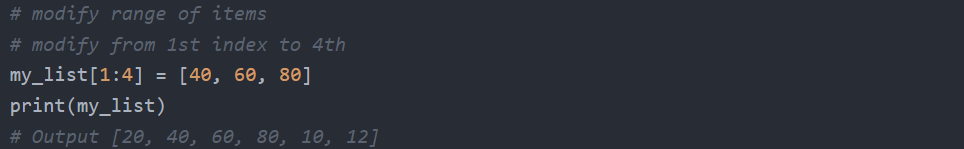
\includegraphics[width=1.0\textwidth]{range-modify-list}
			\caption{Modify range of items.}
			\label{fig:list-range-modify-list}
		\end{figure}
	\item Modify all items.
		\begin{figure}[h]
			\centering
			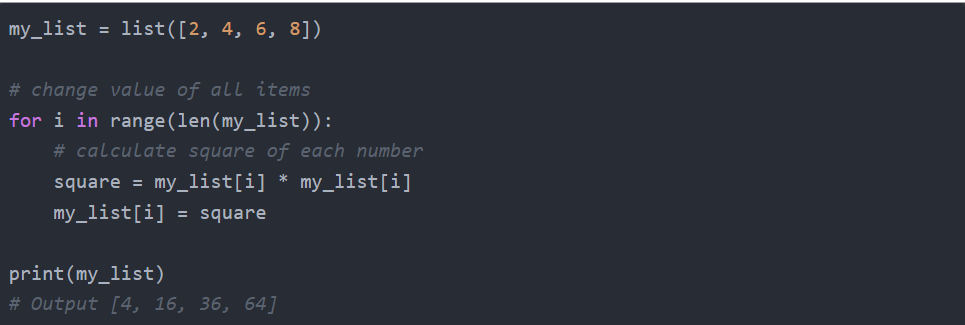
\includegraphics[width=1.0\textwidth]{all-modify-list}
			\caption{Modify a single item.}
			\label{fig:list-all-modify-list}
		\end{figure}
\end{itemize}

\subsection{Removing items from a List}
\begin{table}[h!]
	\centering
	\begin{tabularx}{\textwidth}{|l|X|}
		\hline
		Method & Description \\
		\hline
		remove(item) & To remove THE FIRST OCCURRENCE of the item on the list. \\
		\hline
		pop(index) & Remove and return the item at the given index \\
		\hline
		clear() & To remove all item from the list. The output will be an empty list \\
		\hline
		del listname & Delete entire list \\
		\hline
\end{tabularx}
\caption{List Item Removal Methods in Python}
\label{tab:list-removal}
\end{table}

\subsection{Finding an element in the list}
We can use the index() function to find an item in a list. \\ [0.5em]
{\large Syntax:} The index() func will accept the value of the element as a parameter and returns the first occurrence of the element or returns ValueError if the element does not exist. \\
\newpage

\begin{figure}[h]
	\centering
	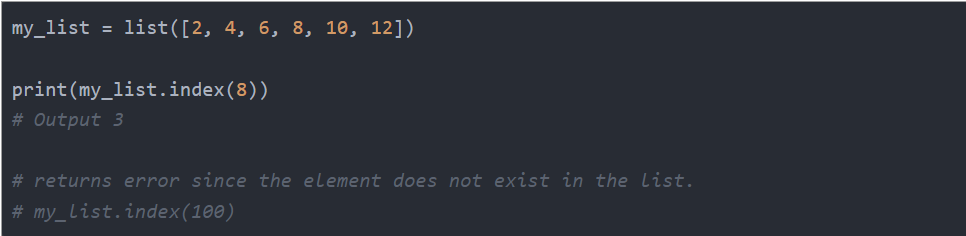
\includegraphics[width=1.0\textwidth]{index-func-list}
	\caption{Examples of using index() func to get find the element in a list.}
	\label{fig:index-func}
\end{figure}

\subsection{Concatenation of two lists}
\begin{itemize}
	\item Using the + operator.
	\item Using the extend() method to append a new list at the end.
\end{itemize}

\begin{figure}[h]
	\centering
	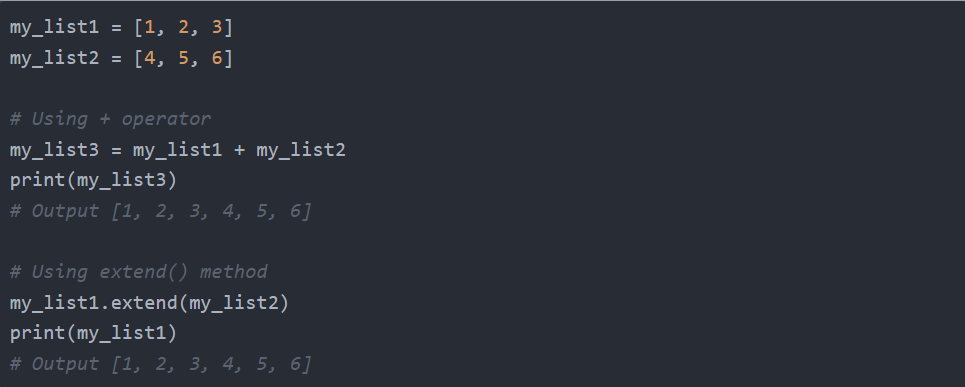
\includegraphics[width=1.0\textwidth]{list-concat}
	\caption{Lists concatenation.}
	\label{fig:list-concat}
\end{figure}

\subsection{Copying a list}
\subsubsection{Using assignment operator (=)}
{\large This is called Deep Copying, the changes made to the original list will be reflected in the new one.}
\newpage

\begin{figure}[h]
	\centering
	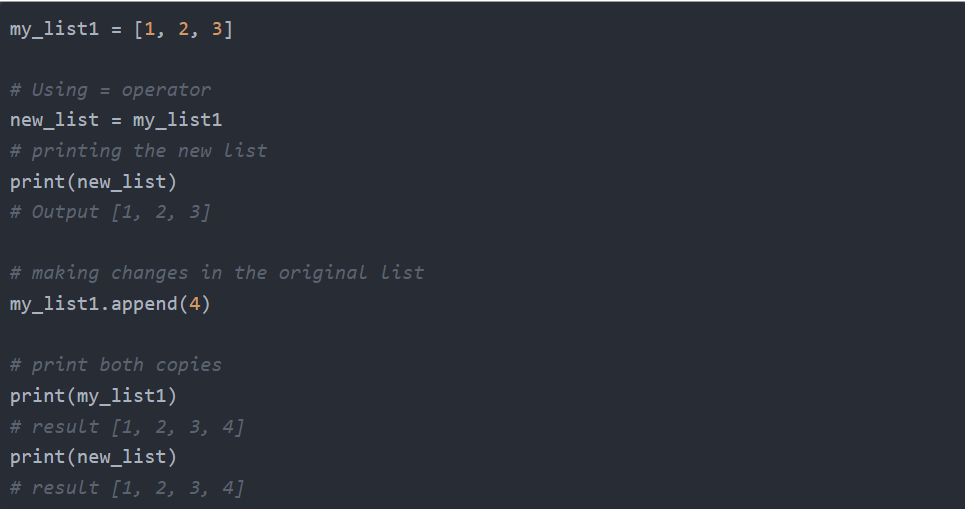
\includegraphics[width=1.0\textwidth]{list-deep-copy}
	\caption{Copying list using assignment operator.}
	\label{fig:list-deep-copy}
\end{figure}

\subsubsection{Using the copy() method}
{\large The copy method can be used to create a copy of a list. This will create a new list and any changes made in the original list will not reflect in the new list. This is shallow copying.}
\newpage

\begin{figure}[h]
	\centering
	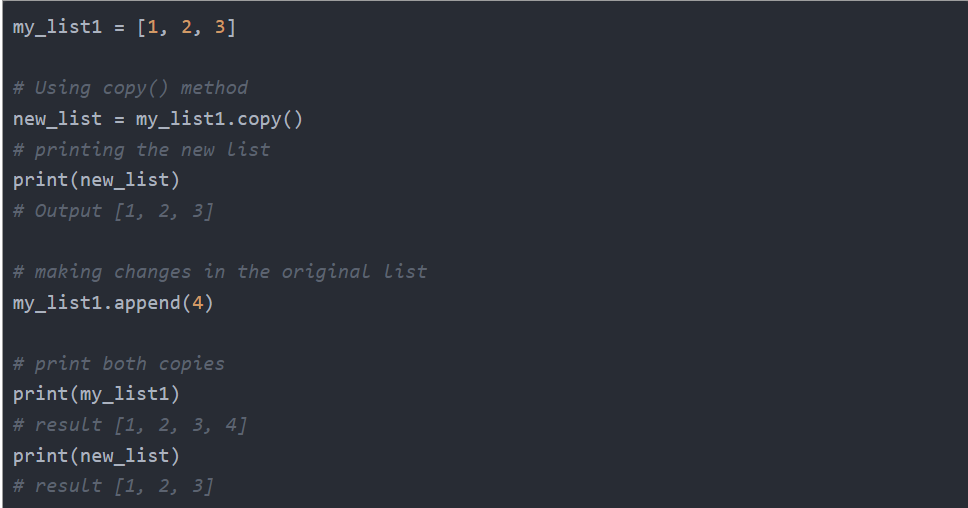
\includegraphics[width=1.0\textwidth]{list-copy-method}
	\caption{Copying list using copy() method.}
	\label{fig:list-shallow-copy}
\end{figure}

\subsection{Sort List using sort()}
The sort function sorts the elements in the list in ascending order.

\begin{figure}[h]
	\centering
	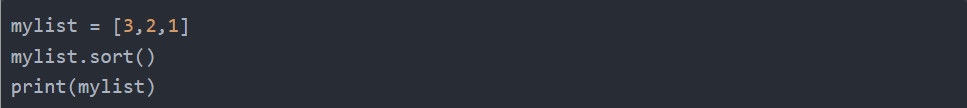
\includegraphics[width=1.0\textwidth]{list-sort-func}
	\caption{Sort a list in ascending order.}
	\label{fig:list-sort-func}
\end{figure}

Output: [1, 2, 3]

\subsection{Reverse a list using reverse()}

\begin{figure}[h]
	\centering
	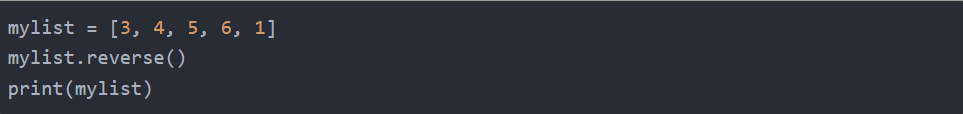
\includegraphics[width=1.0\textwidth]{list-reverse}
	\caption{Reversing a List.}
	\label{fig:list-reverse}
\end{figure}

Output: [1, 6, 5, 4, 3]